\documentclass{article}
\usepackage{tikz}
\usetikzlibrary{positioning, shapes, fit, arrows.meta}
\usepackage{subcaption}

\begin{document}

\begin{figure}
\centering
\begin{subfigure}{0.48\textwidth}
\centering
\begin{tikzpicture}[
    set/.style={draw, ellipse, minimum width=40pt, minimum height=30pt},
    node/.style={circle, fill, inner sep=1.5pt},
    label/.style={font=\footnotesize}
]
    % N[x] and N[y] neighborhoods
    \node[node, label=below:$x$] (x) at (0,0) {};
    \node[node, label=below:$y$] (y) at (1.5,0) {};
    \node[set, fit=(x), label=above:$N[x]$] (nx) {};
    \node[set, fit=(y), label=above:$N[y]$] (ny) {};
    
    % S set partially outside
    \node[set, draw=red, label=above:$S$, minimum width=60pt] (S) at (0.75,0.75) {};
    \node[node] at (S.west) {};
    \node[node] at (S.south) {};
    
    % Z set with |Z| ≥ 5
    \node[set, label=below:$Z$, minimum width=80pt] (Z) at (0.75,-1) {};
    \foreach \i in {1,...,5} {
        \node[node, label=below:$z_\i$] at (Z.south west+\i*0.4) {};
    }
    
    % Visualize union boundaries
    \draw[dashed, gray!50] (nx.north west) -- (ny.north east);
    \draw[dashed, gray!50] (nx.south west) -- (ny.south east);
\end{tikzpicture}
\caption{Case $S \nsubseteq N[x] \cup N[y]$ and $|Z| \geq 5$}
\end{subfigure}
\hfill
\begin{subfigure}{0.48\textwidth}
\centering
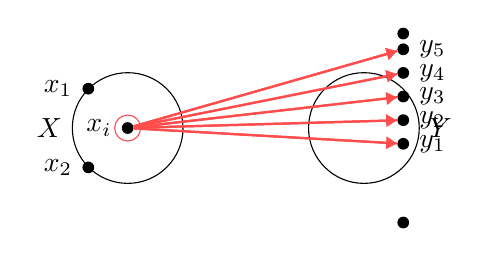
\begin{tikzpicture}[
    set/.style={draw, circle, minimum size=40pt},
    node/.style={circle, fill, inner sep=1.5pt},
    edge/.style={thick, red!70}
]
    % X and Y vertex sets
    \node[set, label=left:$X$] (X) at (0,0) {};
    \node[set, label=right:$Y$] (Y) at (3,0) {};
    
    % X vertices
    \node[node, label=left:$x_1$] (x1) at (-0.5,0.5) {};
    \node[node, label=left:$x_2$] (x2) at (-0.5,-0.5) {};
    \node[node, label=left:$x_i$] (xi) at (0,0) {};
    
    % Y vertices with 5 neighbors
    \foreach \i in {1,...,5} {
        \node[node, label=right:$y_\i$] (y\i) at (3.5, -0.5+\i*0.3) {};
        \draw[edge] (xi) -- (y\i);
    }
    
    % Other Y vertices
    \node[node] (y6) at (3.5,-1.2) {};
    \node[node] (y7) at (3.5,1.2) {};
    
    % Highlight x_i and connections
    \node[circle, draw=red!70, fit=(xi), inner sep=1pt] {};
    \draw[edge, -{Triangle[scale=0.8]}] (xi) -- (y1);
    \draw[edge, -{Triangle[scale=0.8]}] (xi) -- (y2);
    \draw[edge, -{Triangle[scale=0.8]}] (xi) -- (y3);
    \draw[edge, -{Triangle[scale=0.8]}] (xi) -- (y4);
    \draw[edge, -{Triangle[scale=0.8]}] (xi) -- (y5);
\end{tikzpicture}
\caption{Contradiction setup in Claim 3}
\end{subfigure}
\end{figure}

\end{document}